% Generated by src/tools/c-f16-certified-square.py from evidence/figures/c-f16-certified-square.csv. Do not edit.
\node[anchor=south west, inner sep=0] at (0,0) {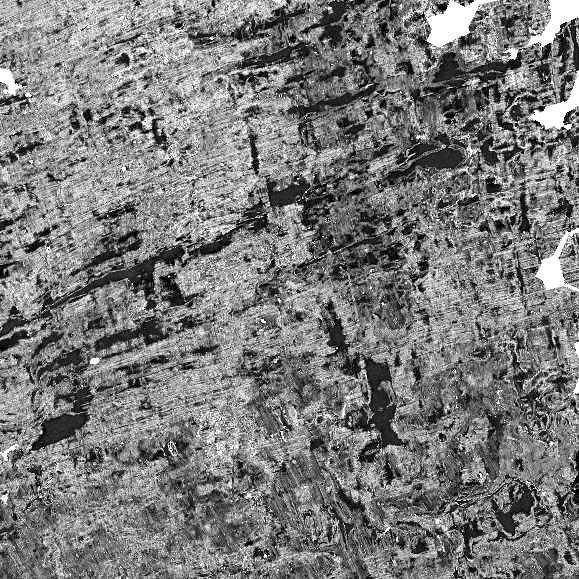
\includegraphics[width=8.4000cm,height=8.4000cm]{../paper/figures/assets/c-f16-certified-square-texture.png}};
\node[anchor=south west, inner sep=0] at (8.9500,0) {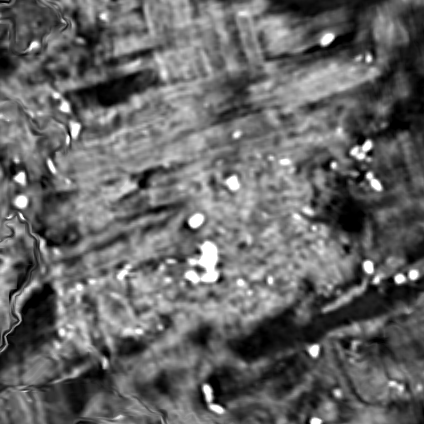
\includegraphics[width=8.4000cm,height=8.4000cm]{../paper/figures/assets/c-f16-certified-square-zoom.png}};
\draw[saorange, line width=1.1pt] (0.8705,0.8705) rectangle (7.5295,7.5295);
\draw[sasky, line width=1.1pt] (0.9865,1.7554) rectangle (6.9492,7.7181);
\draw[white, line width=1.6pt] (3.8881,4.3959) rectangle (4.6570,5.1648);
\draw[black, line width=0.6pt] (3.8881,4.3959) rectangle (4.6570,5.1648);
\draw[white, line width=1.3pt] (4.6570,5.1648) -- (8.9500,8.4000);
\draw[white, line width=1.3pt] (4.6570,4.3959) -- (8.9500,0);
\draw[black, line width=0.45pt] (4.6570,5.1648) -- (8.9500,8.4000);
\draw[black, line width=0.45pt] (4.6570,4.3959) -- (8.9500,0);
\draw[black, line width=0.6pt] (8.9500,0) rectangle (17.3500,8.4000);
\fill[white, opacity=0.85] (6.0602,0.12) rectangle (8.3000,0.78);
\fill[black] (6.2102,0.25) rectangle (8.1500,0.33);
\node[font=\footnotesize, anchor=south, inner sep=1pt] at (7.1801,0.34) {5 mm};
\fill[white, opacity=0.85] (14.8309,0.12) rectangle (17.2500,0.78);
\fill[black] (14.9809,0.25) rectangle (17.1000,0.33);
\node[font=\footnotesize, anchor=south, inner sep=1pt] at (16.0404,0.34) {0.5 mm};
\node[anchor=north west, fill=white, fill opacity=0.88, text opacity=1, font=\footnotesize, align=left, inner sep=3pt] at (0.18,8.2200) {\tikz[baseline=-0.6ex]\draw[sasky, line width=1.1pt] (0,-0.1) rectangle (0.32,0.1); certified square, 15.3693 mm\\\tikz[baseline=-0.6ex]\draw[saorange, line width=1.1pt] (0,-0.1) rectangle (0.32,0.1); hole free square, 17.1642 mm\\\tikz[baseline=-0.6ex]\draw[black, line width=0.6pt] (0,-0.1) rectangle (0.32,0.1); window shown at right, 1.98 mm};
\node[anchor=south west, fill=white, fill opacity=0.88, text opacity=1, font=\footnotesize, inner sep=2pt] at (0.18,0.18) {raw scan, no ink detector};
\node[anchor=north west, fill=white, fill opacity=0.88, text opacity=1, font=\footnotesize, inner sep=2pt] at (9.1300,8.2200) {10.9$\times$, resampled from the raw scan};
